\documentclass{article}
\usepackage{tikz}
\usepackage{caption}

\begin{document}

\begin{figure}[h]
    \centering
    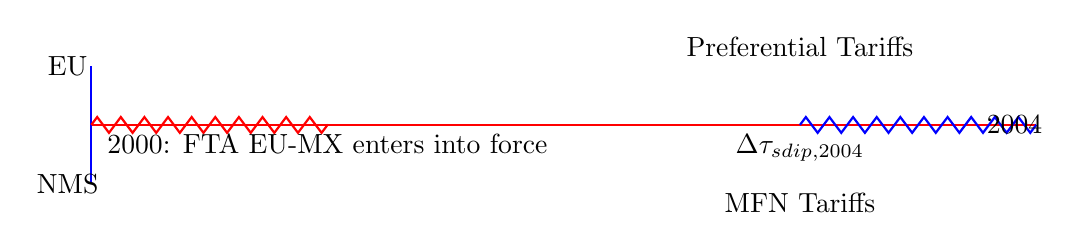
\begin{tikzpicture}[scale=1.5]
        % Draw the horizontal line
        \draw[thick, red] (0,0) -- (8,0);
        
        % Draw the vertical line
        \draw[thick, blue] (0,-0.5) -- (0,0.5);
        
        % Label the vertical line
        \node at (-0.2, 0.5) {EU};
        \node at (-0.2, -0.5) {NMS};
        
        % Draw the zigzag lines
        \draw[thick, red, decorate, decoration={zigzag, segment length=3mm, amplitude=1mm}] (0,0) -- (2,0);
        \draw[thick, blue, decorate, decoration={zigzag, segment length=3mm, amplitude=1mm}] (6,0) -- (8,0);
        
        % Add text labels
        \node at (2,0) [below] {2000: FTA EU-MX enters into force};
        \node at (6,0) [below] {$\Delta \tau_{sdip,2004}$};
        \node at (6,0.5) [above] {Preferential Tariffs};
        \node at (6,-0.5) [below] {MFN Tariffs};
        \node at (7.5,0) [right] {2004};
    \end{tikzpicture}
    \caption{\textbf{Event Study Design, Constructing the Trade Shock}: I use the fact that when the NMS joined the EU in 2004, they had immediate preferential access to third-party markets via previously signed EU trade agreements which the NMS did not get to negotiate. The product-level bilateral tariff variation $\Delta \tau_{sdip,2004}$ which was a by-product of the EU accession process is my measure of the market accession shock. In the example above, the EU joined a FTA with Mexico in 2000, but the NMS only joined the EU in 2004, so in 2004 they immediately adhered to these previously negotiated tariff schedules.}
    \label{fig:event_study_design}
\end{figure}

\end{document}